\begin{frame}{Theory: Topological insulator}
	2005 Kane and Mele found another class of material: \\the topological insulator (TI).
	\\
	\begin{columns}
		\begin{column}<2->{0.33\linewidth}
			spin-orbit coupling
		\end{column}
		\hspace{-1cm}
		\begin{column}<3->{0.33\linewidth}
			$\rightarrow$ band inversion
		\end{column}
		\hspace{-1.2cm}
		\begin{column}<4->{0.33\linewidth}
			$\rightarrow$ Dirac cone
		\end{column}
	\end{columns}
	\begin{columns}
		\begin{column}<5->{.5\linewidth}
			\begin{figure}
				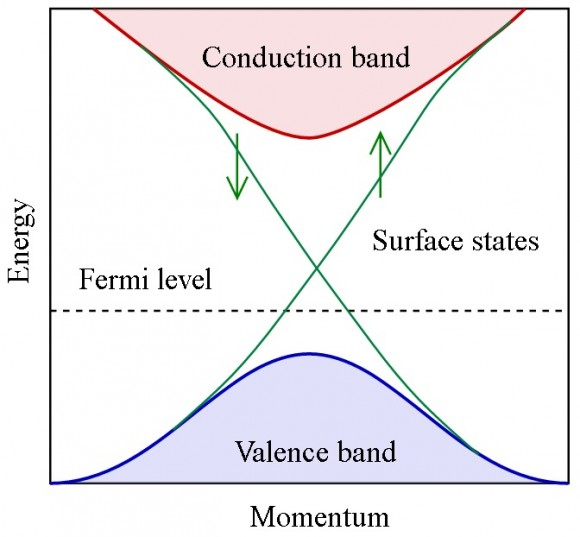
\includegraphics[width=\textwidth]{andere_bilder/band_structure_top_insulator}
			\end{figure}
		\end{column}
		\begin{column}{.5\linewidth}
			\begin{block}<6->{2D TI: }
			have quantum spin edge states found in graphene and HgTe quantum wells.
			\end{block}
			\begin{block}<7->{3D TI: }
			strong and weak ones \\
			HgTe is semi metal but under strain $\Gamma_6$ and $\Gamma_8$ bands can close up at Fermi level. 
			\end{block}
		\end{column}
	\end{columns}
	
\end{frame}

\begin{frame}{Theory: Crystal description}

	\begin{block}{Translation Vector: $\boldsymbol{R}_i = x_i \boldsymbol{a}_1 + y_i \boldsymbol{a}_2 + z_i \boldsymbol{a}_3$}
		contains basis for lattice forming a unit cell. \\
		Smallest primitive unit cell is the Wigner Seitz cell.
	\end{block}
	\begin{columns}
		\begin{column}{0.3\linewidth}
			Bravais lattice  
		\end{column}
	\end{columns}
	\begin{columns}
		\begin{column}{0.5\linewidth}
			fcc lattice with two atomic basis 
		\end{column}
		\hspace{-1cm}
		\begin{column}{0.55\linewidth}
			$\rightarrow$ diamond or zinc-blende structure 
		\end{column}
	\end{columns}
	\begin{columns}
		\begin{column}{.25\linewidth}
			\centering
			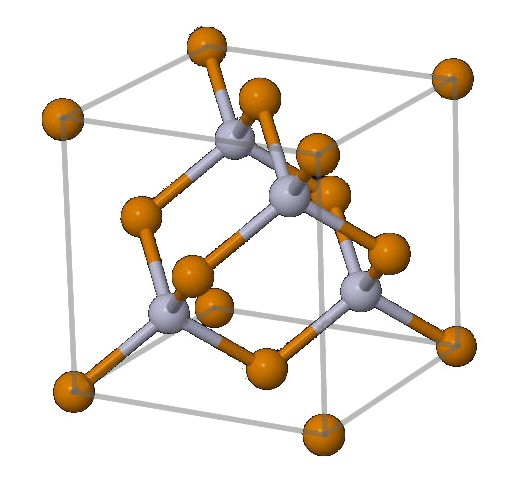
\includegraphics[width=\linewidth]{andere_bilder/zinc_blende}
		\end{column}
		\hfill
		\begin{column}{.25\linewidth}
			\centering
			\begin{tabular}{c c c c} 
				\hline
				& \textbf{x} & \textbf{y} & \textbf{z}\\ 
				\hline 
				\vspace{0.2cm} 
				$\boldsymbol{a}_1$ & 0 & $\frac{a}{2}$ & $\frac{a}{2}$ \\
				\vspace{0.2cm}
				$\boldsymbol{a}_2$ & $\frac{a}{2}$ & 0 & $\frac{a}{2}$ \\
				\vspace{0.2cm}
				$\boldsymbol{a}_3$ & $\frac{a}{2}$ & $\frac{a}{2}$ & 0 \\
%			\end{tabular}	
%		\end{minipage}
%		\\
%		\begin{minipage}[c]{.33\linewidth}
%			\begin{tabular}{c c c c} 
%				\hline
%				& \textbf{x} & \textbf{y} & \textbf{z}\\ 
				\hline 
				\vspace{0.2cm}
				atom & 0 & 0 & 0 \\
				\vspace{0.2cm}
				atom & $\frac{a}{4}$ & $\frac{a}{4}$ & $\frac{a}{4}$
			\end{tabular}	
		\end{column}
		\begin{column}{.5\linewidth}
			bla
		\end{column}
	\end{columns}
\end{frame}

\begin{frame}{Theory: Surface modeling}
	blub
\end{frame}

\begin{frame}{Theory: DFT and SOC}
	blub
\end{frame}
%%% Local Variables:
%%% mode: latex
%%% TeX-master: "main_BA2_Vortrag.tex"
%%% End: